% =====================================================================
%  XrVit course paper -- IEEE conference format (two columns)
%  Compile on Overleaf (pdfLaTeX) or locally with:
%     pdflatex main && bibtex main && pdflatex main && pdflatex main
% =====================================================================
\documentclass[conference]{IEEEtran}

\usepackage{cite}
\usepackage{amsmath,amssymb}
\usepackage{graphicx}
\usepackage{booktabs}
\usepackage{multirow}
\usepackage{xcolor}
\usepackage{tikz}
\usetikzlibrary{positioning,arrows.meta,fit,calc}
\usepackage{pgfplots}
\pgfplotsset{compat=1.18}
\usepackage{url}
\usepackage[hidelinks]{hyperref}
\usepackage[capitalise]{cleveref}

% Marks text the authors must fill in. Remove before submission.
\newcommand{\authornote}[1]{\textbf{\textcolor{blue}{[#1]}}}
\newcommand{\ns}{\textsuperscript{n.s.}}

\begin{document}

\title{Distilling a Chest X-ray Foundation Model Ensemble into a Lightweight CNN: Near-RAD-DINO Accuracy at 5.7$\times$ Lower Inference Cost}

\author{
\IEEEauthorblockN{\authornote{Author 1}, \authornote{Author 2}}
\IEEEauthorblockA{\authornote{Department, University}\\
\authornote{City, Country}\\
\authornote{email}}
}

\maketitle

% =====================================================================
\begin{abstract}
Chest X-ray foundation models such as RAD-DINO classify thoracic findings more accurately than small convolutional neural networks (CNNs), but they are expensive to run. We show that most of this advantage can be moved into a lightweight CNN through knowledge distillation. A ConvNeXt-Tiny and a RAD-DINO model, both fine-tuned on NIH ChestX-ray14, are calibrated and averaged into a teacher ensemble. This ensemble is the most accurate system we tested (macro AUROC 0.8428), but it costs more than RAD-DINO alone. A new ConvNeXt-Tiny student is trained on the ensemble's soft labels with exactly the recipe of the original CNN, and only the student runs at test time. We evaluated on the official test split (25,596 images, 14 findings), with patient-level bootstrap confidence intervals and decision rules fixed in advance. The student raised macro AUROC from 0.8263 to 0.8339 (+0.0076, 95\% CI +0.0058 to +0.0096) at identical inference cost, and it also improved AUPRC, macro F1, recall and precision. Its macro AUROC was within 0.0025 of RAD-DINO (0.8364; difference not significant), its macro recall reached RAD-DINO's, and it ran 5.7$\times$ faster in batch inference on a Tesla T4. The student closed about 75\% of the AUROC gap between the CNN and RAD-DINO. Knowledge distillation therefore offers a practical way to approach foundation-model accuracy on chest X-rays at the cost of a small CNN.
\end{abstract}

\begin{IEEEkeywords}
chest X-ray, knowledge distillation, foundation model, ensemble, efficient inference, multi-label classification
\end{IEEEkeywords}

% =====================================================================
\section{Introduction}
\label{sec:intro}

The chest radiograph (chest X-ray, CXR) is the most commonly ordered imaging test for suspected lung disease~\cite{raoof2012interpretation}. In many health systems, the number of radiologists available to read these images has not kept pace with demand~\cite{rcr2025census}. Deep learning for automated CXR interpretation has therefore become a large research area~\cite{calli2021deep}. Public datasets such as NIH ChestX-ray14, with 112,120 frontal radiographs labelled for 14 findings~\cite{wang2017chestxray8}, made it possible to train CNNs for this task~\cite{rajpurkar2017chexnet}.

More recently, \emph{foundation models} have been built specifically for radiographs. These are large networks pretrained on broad data and then adapted to many tasks~\cite{moor2023foundation}. RAD-DINO is a Vision Transformer (ViT-B/14) pretrained on chest X-rays with the self-supervised DINOv2 method~\cite{perezgarcia2025raddino,oquab2024dinov2}. Its accuracy comes at a price. It has 86.6\,M parameters and reads $518\times518$ pixel inputs, which gives 1,369 image patches whose pairwise attention must be computed~\cite{dosovitskiy2021vit}. A modern CNN such as ConvNeXt-Tiny~\cite{liu2022convnext} has 27.8\,M parameters and works well at $384\times384$ pixels. On the GPU used in this study, RAD-DINO needed 22.8\,ms per image in batches of 32, against 4.0\,ms for ConvNeXt-Tiny.

Several approaches aim to keep a large model's accuracy at a lower cost. Cascades route inputs between a cheap and an expensive model at test time~\cite{wang2018idk,wang2022wisdom}, but they keep both models in deployment. Ensembles of different models are often more accurate than any single member~\cite{dietterich2000ensemble,lakshminarayanan2017deep}, but they multiply the cost. \emph{Knowledge distillation} (KD) avoids both problems. A small student is trained to reproduce the soft predictions of a stronger teacher, and only the student is run afterwards~\cite{bucilua2006model,hinton2015distilling,gou2021knowledge}. Its inference cost is fixed and equal to that of the student.

This paper combines the two ideas. We use the ensemble of a CNN and RAD-DINO as the teacher, and distil it into a single ConvNeXt-Tiny. Our contributions are:
\begin{enumerate}
  \item We show that ConvNeXt-Tiny and RAD-DINO are complementary on the official ChestX-ray14 test split: their calibrated average is significantly more accurate than either model alone.
  \item We distil this two-model teacher into one ConvNeXt-Tiny, trained with exactly the recipe of the original CNN. The distilled student is significantly more accurate than the CNN at the same cost, and it comes within 0.0025 macro AUROC of RAD-DINO at 5.7$\times$ lower batch cost. All decision rules were fixed before the experiment.
  \item We analyse per finding where the student gains, and how it recovers positives that only RAD-DINO had found.
\end{enumerate}

% =====================================================================
\section{Related Work}
\label{sec:related}

\subsection{Chest X-ray Classification and Foundation Models}
CNNs trained on ChestX-ray14, such as CheXNet~\cite{rajpurkar2017chexnet}, established the dataset as a standard benchmark~\cite{calli2021deep}. Its labels were mined from report text and contain errors~\cite{oakdenrayner2020exploring}. Models trained on one population can also perform worse on another~\cite{zech2018variable}, so results from different data splits are not directly comparable. Self-supervised foundation models trained on radiographs, such as RAD-DINO~\cite{perezgarcia2025raddino}, provide stronger starting features than networks pretrained on natural images~\cite{deng2009imagenet}, but their inference cost is rarely reported next to their accuracy.

\subsection{Ensembles}
Combining the predictions of several models usually improves accuracy, especially when the members make different errors~\cite{dietterich2000ensemble}. Averaging the outputs of independently trained deep networks is a simple and strong baseline~\cite{lakshminarayanan2017deep}. The price is that every member must be run on every input.

\subsection{Knowledge Distillation}
Distillation was introduced as model compression~\cite{bucilua2006model} and popularised with temperature-softened teacher outputs~\cite{hinton2015distilling}; a survey is given in~\cite{gou2021knowledge}. Distilling an ensemble into one network was one of the original motivations~\cite{bucilua2006model,hinton2015distilling}. Soft targets can also reduce the effect of noisy labels~\cite{li2017noisy}, and even a student with the same architecture as its teacher can improve on it~\cite{furlanello2018born}. Larger teachers do not always make better students~\cite{cho2019efficacy,mirzadeh2020teacher}. For CXRs, Ho and Gwak distilled larger CNNs into lightweight students on ChestX-ray14~\cite{ho2020utilizing}. Termritthikun et~al.\ compared CNN and transformer teachers for an on-device student~\cite{termritthikun2024explainable}, and Kishore et~al.\ distilled a self-supervised teacher into a compressed student~\cite{kishore2025enhancing}. We did not find a study that distils RAD-DINO, or an ensemble containing it, into a CNN.

% =====================================================================
\section{Methods}
\label{sec:methods}

\Cref{fig:pipeline} summarises the method: two trained models form a teacher ensemble, the ensemble labels the training images with soft probabilities, and a new CNN learns from these labels. Only the student runs at test time.

\begin{figure}[t]
\centering
\resizebox{\columnwidth}{!}{%
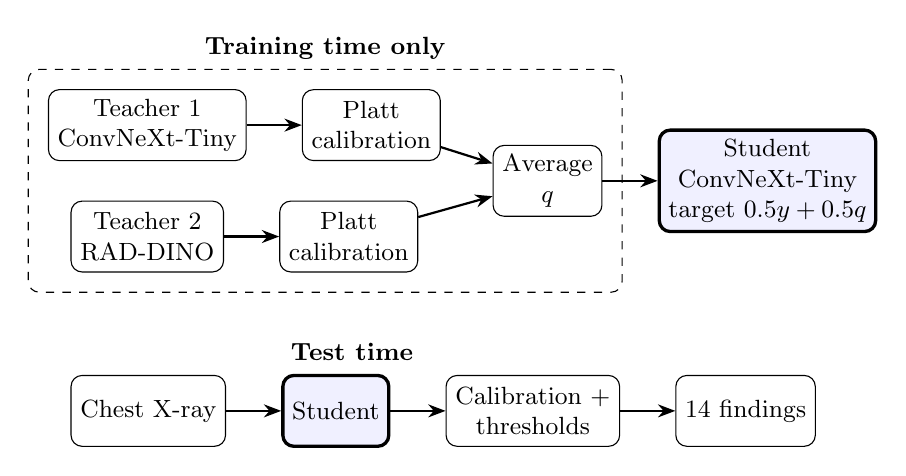
\begin{tikzpicture}[
  node distance=5mm and 7mm,
  box/.style={draw, rounded corners, align=center, minimum height=9mm, font=\small},
  hl/.style={box, very thick, fill=blue!6},
  arr/.style={-{Stealth[length=2.2mm]}, thick}
]
  \node[box] (cnn) {Teacher 1\\ConvNeXt-Tiny};
  \node[box, below=of cnn] (rd) {Teacher 2\\RAD-DINO};
  \node[box, right=of cnn] (c1) {Platt\\calibration};
  \node[box, right=of rd] (c2) {Platt\\calibration};
  \coordinate (mid) at ($(c1.east)!0.5!(c2.east)$);
  \node[box, right=8mm of mid] (avg) {Average\\$q$};
  \node[hl, right=of avg] (st) {Student\\ConvNeXt-Tiny\\target $0.5y + 0.5q$};
  \node[draw, dashed, rounded corners, inner sep=2.5mm, fit=(cnn)(rd)(c1)(c2)(avg),
        label={[font=\small\bfseries]above:Training time only}] {};
  \node[box, below=13mm of rd.south west, anchor=north west] (x) {Chest X-ray};
  \node[hl, right=of x] (st2) {Student};
  \node[box, right=of st2] (dec) {Calibration +\\thresholds};
  \node[box, right=of dec] (y) {14 findings};
  \node[font=\small\bfseries, above=0.5mm of st2.north west, anchor=south west] {Test time};
  \draw[arr] (cnn) -- (c1);
  \draw[arr] (rd) -- (c2);
  \draw[arr] (c1) -- (avg);
  \draw[arr] (c2) -- (avg);
  \draw[arr] (avg) -- (st);
  \draw[arr] (x) -- (st2);
  \draw[arr] (st2) -- (dec);
  \draw[arr] (dec) -- (y);
\end{tikzpicture}}
\caption{Distillation pipeline. The two calibrated teachers are averaged into soft labels $q$ for the training images. The student learns from $q$ and the real labels $y$. At test time only the student runs, at the cost of the original CNN.}
\label{fig:pipeline}
\end{figure}

\subsection{Data}
We use NIH ChestX-ray14~\cite{wang2017chestxray8}, which contains frontal radiographs labelled for 14 findings. The task is multi-label: an image can carry several findings, and an image with no finding has an all-zero label vector. The official test list is kept unchanged. A validation set is drawn from 15\% of the official train/validation \emph{patients}, so that no patient appears in more than one partition. The split is fixed by SHA-256 hashes that every experiment checks. \Cref{tab:data} shows that the official test population is harder than the development data. It has more findings per image and fewer standard posterior--anterior (PA) views.

\begin{table}[t]
\centering
\caption{Data partitions. The official test set carries more findings per image than the training and validation data.}
\label{tab:data}
\begin{tabular}{@{}lrrr@{}}
\toprule
 & Train & Validation & Test \\
\midrule
Images           & 73,916 & 12,608 & 25,596 \\
Patients         & 23,806 & 4,202  & 2,797 \\
Images per patient & 3.1 & 3.0 & 9.2 \\
Findings per image & 0.63 & 0.61 & 1.06 \\
Images with no finding & 58\% & 59\% & 39\% \\
PA views         & 65\% & 66\% & 43\% \\
\bottomrule
\end{tabular}
\end{table}

\subsection{Teacher Models}
\textbf{CNN.} ConvNeXt-Tiny~\cite{liu2022convnext}, pretrained on ImageNet-22k and fine-tuned on ImageNet-1k~\cite{deng2009imagenet}, with $384\times384$ input. The head consists of global average pooling, dropout 0.2 and a linear layer to 14 outputs. After one epoch that trains only the head, the whole network is fine-tuned for up to 8 epochs (learning rate $10^{-4}$, batch 32, stochastic depth 0.1).

\textbf{RAD-DINO.} ViT-B/14 from~\cite{perezgarcia2025raddino}, with $518\times518$ input. The CLS token is concatenated with the mean patch token and passed through dropout 0.2 and a linear layer. The model first trains only the head for 2 epochs. The last 8 of its 12 transformer blocks are then fine-tuned for up to 4 epochs with layer-wise learning-rate decay (0.8). The evaluated weights are an exponential moving average (decay 0.999).

\textbf{Shared recipe.} All networks, including the student, use the Asymmetric Loss (ASL)~\cite{ridnik2021asl} with $\gamma_+=1$, $\gamma_-=4$ and margin 0.05. This loss down-weights the many easy negatives of rare findings. Training uses AdamW with cosine decay, mixed precision and light augmentation (random resized crop, horizontal flip, $\pm7^\circ$ rotation, brightness/contrast jitter). Early stopping uses validation macro AUROC. Each model is trained once, with seed 42, on one NVIDIA Tesla T4.

\subsection{Calibration and Decision Thresholds}
For each finding $c$, the raw logit $z_c$ is turned into a probability with Platt scaling~\cite{platt1999probabilistic},
\begin{equation}
\hat{p}_c = \sigma(a_c z_c + b_c),
\label{eq:platt}
\end{equation}
where $a_c$ and $b_c$ are fitted on validation by minimising the negative log-likelihood. Calibration puts the two teachers on the same probability scale before they are averaged~\cite{guo2017calibration}. Each finding then gets its own yes/no threshold, chosen to maximise F1 on validation. All fitted values are applied unchanged to the test set.

\subsection{Teacher Ensemble}
The teacher is the equal-weight average of the two calibrated models:
\begin{equation}
q_{i,c} = \tfrac{1}{2}\left(\hat{p}^{\,\text{CNN}}_{i,c} + \hat{p}^{\,\text{RAD-DINO}}_{i,c}\right).
\label{eq:teacher}
\end{equation}
The equal weights were fixed in advance. The same average is also evaluated as a system of its own (``Average''), which shows how accurate the teacher is.

\subsection{Knowledge Distillation}
\textbf{Soft labels.} $q$ is computed once for the 73,916 training images, without augmentation. Validation and test images never receive soft labels.

\textbf{Go/no-go check.} The teachers were trained on the same images, so their soft labels might simply copy the real labels. We fixed in advance that the student would be trained only if the teacher's macro AUROC on the training images was below 0.95.

\textbf{Student.} The student is a new ConvNeXt-Tiny, initialised from ImageNet (not from the trained CNN) and trained with exactly the recipe of the original CNN. Only the training target changes:
\begin{equation}
t_{i,c} = (1-\lambda)\,y_{i,c} + \lambda\,q_{i,c}, \qquad \lambda = 0.5 .
\label{eq:target}
\end{equation}
Because ASL is linear in its target, this is equal to averaging the loss against the real label $y$ and the loss against the teacher $q$. Any difference between the student and the original CNN therefore comes from the teacher alone. At test time the student is followed by its own calibration~\eqref{eq:platt} and thresholds.

\subsection{Evaluation}
\textbf{Metrics.} The primary metric is macro AUROC, the mean over the 14 findings of the area under the ROC curve~\cite{hanley1982meaning}. Secondary metrics are macro AUPRC, macro and micro F1, and recall and precision at the fitted thresholds.

\textbf{Uncertainty.} 95\% confidence intervals come from 1,000 bootstrap resamples of test \emph{patients}~\cite{efron1993bootstrap}. Resampling patients matters because test patients have 9.2 images on average. Systems are compared on the same resamples. A difference is called significant only if its CI excludes zero \emph{and} its Holm-corrected~\cite{holm1979simple} two-sided $p<0.05$. The Holm correction covers the three student comparisons within each metric. The baseline comparisons were corrected over six pairwise comparisons in the original evaluation, which is conservative.

\textbf{Outcome rules} (fixed before the distillation run, on test macro AUROC). The student \emph{helps} if it is significantly better than the CNN. It \emph{matches} RAD-DINO if the lower CI bound of (student $-$ RAD-DINO) lies above $-0.005$, i.e.\ half of the CNN-to-RAD-DINO gap. It \emph{beats} RAD-DINO if it is significantly better than RAD-DINO.

\textbf{Inference cost.} We measure forward-pass time per image on a Tesla T4 in fp16, at batch sizes 1 and 32 (50 warm-up and 200 timed iterations, median of 3 repeats). Image loading and resizing are excluded.

% =====================================================================
\section{Results}
\label{sec:results}

\subsection{Main Accuracy--Efficiency Comparison}

The central comparison is between the original CNN, RAD-DINO, their prediction-level ensemble, and the distilled CNN. \Cref{fig:latency} plots macro AUROC against measured batch-32 inference latency for all four systems, with marker area proportional to parameter count, and \cref{tab:main} gives the exact values on the 25,596-image test set. RAD-DINO improved macro AUROC over the CNN by 0.0101 (0.8364 vs.\ 0.8263), but required substantially more inference time from a model with 3.1$\times$ as many parameters (86.6\,M vs.\ 27.8\,M). The distilled CNN reached 0.8339 macro AUROC, improving over the CNN by 0.0076 while retaining the CNN's measured inference cost and parameter count. As \cref{fig:latency} shows, the student is the only system that moves up from the CNN's accuracy without moving right in cost or growing in size.

\begin{figure}[t]
\centering
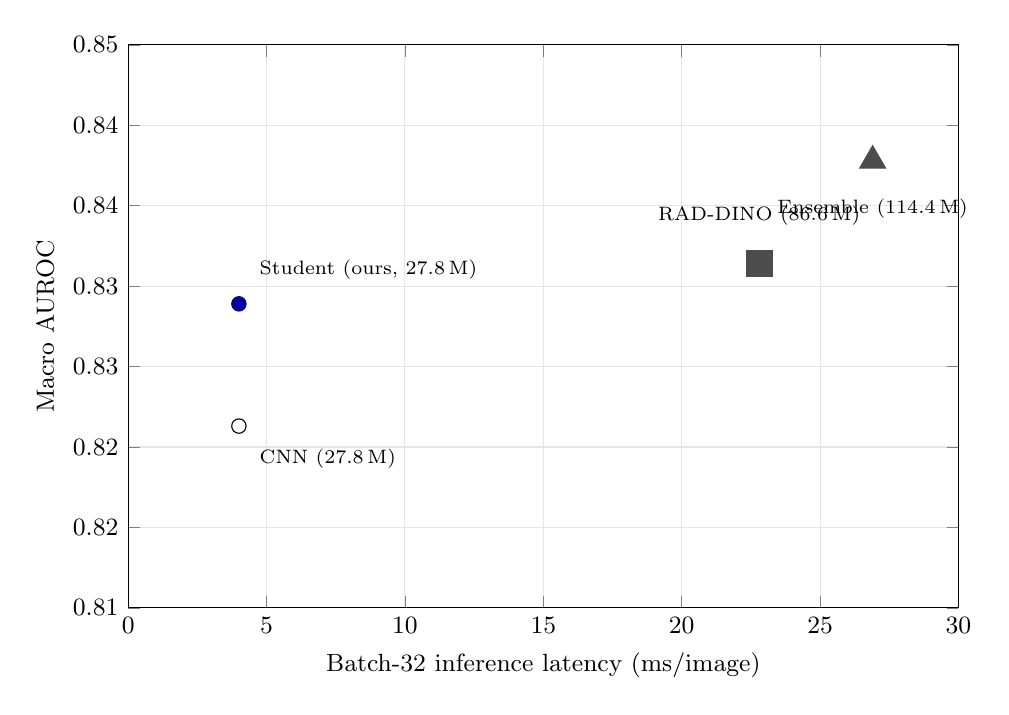
\begin{tikzpicture}
\begin{axis}[
  width=\columnwidth,
  height=0.72\columnwidth,
  xlabel={Batch-32 inference latency (ms/image)},
  ylabel={Macro AUROC},
  xmin=0, xmax=30,
  ymin=0.815, ymax=0.850,
  tick label style={font=\small},
  label style={font=\small},
  xmajorgrids, ymajorgrids,
  grid style={gray!20},
  clip=false,
]
\addplot[only marks, mark=o, mark size=2.6pt, color=black] coordinates {(4.0,0.8263)};
\addplot[only marks, mark=*, mark size=2.6pt, color=blue!60!black] coordinates {(4.0,0.8339)};
\addplot[only marks, mark=square*, mark size=4.7pt, color=gray!60!black] coordinates {(22.8,0.8364)};
\addplot[only marks, mark=triangle*, mark size=5.4pt, color=gray!60!black] coordinates {(26.9,0.8428)};
\node[anchor=north west, font=\scriptsize] at (axis cs:4.4,0.8255) {CNN (27.8\,M)};
\node[anchor=south west, font=\scriptsize] at (axis cs:4.4,0.8348) {Student (ours, 27.8\,M)};
\node[anchor=south, font=\scriptsize] at (axis cs:22.8,0.8382) {RAD-DINO (86.6\,M)};
\node[anchor=north, font=\scriptsize] at (axis cs:26.9,0.8410) {Ensemble (114.4\,M)};
\end{axis}
\end{tikzpicture}
\caption{Macro AUROC versus measured batch-32 inference latency (Tesla T4, fp16); marker area is proportional to parameter count (CNN and Student 27.8\,M, RAD-DINO 86.6\,M, Ensemble 114.4\,M, both networks run). The student reaches near-RAD-DINO accuracy at the CNN's inference cost and size.}
\label{fig:latency}
\end{figure}

\Cref{fig:metrics} shows that the same pattern holds across the threshold-independent ranking metrics. Relative to the CNN, the student increased macro AUPRC from 0.2988 to 0.3146 and macro F1 from 0.3539 to 0.3702. Its macro recall increased from 0.4304 to 0.4622, while precision increased from 0.3188 to 0.3326. RAD-DINO remained stronger on micro F1 (0.4317 vs.\ 0.4192, omitted from \cref{fig:metrics} for scale reasons and reported in \cref{tab:main} instead), indicating that the student's gains were not uniform across all evaluation criteria. At batch size 32, the student was 5.7$\times$ faster than RAD-DINO (4.0 vs.\ 22.8\,ms per image); at batch size 1, the corresponding measurements were 11.4 and 22.2\,ms per image.

\begin{figure}[t]
\centering
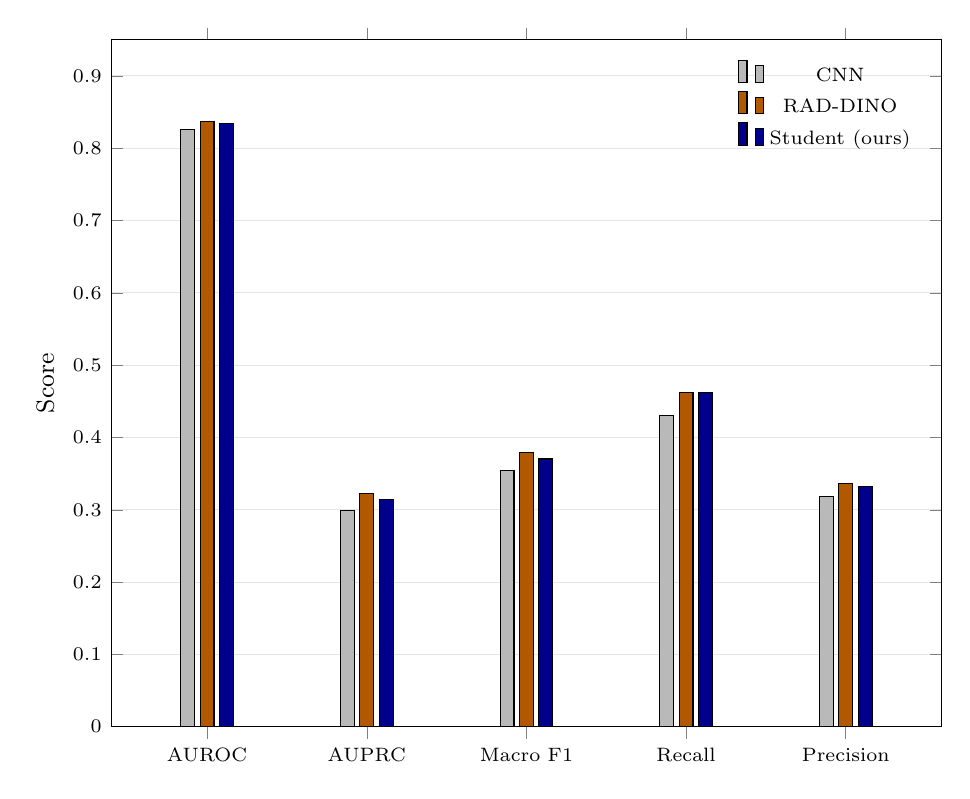
\begin{tikzpicture}
\begin{axis}[
  width=\columnwidth,
  height=0.85\columnwidth,
  ybar,
  bar width=5pt,
  ymin=0, ymax=0.95,
  symbolic x coords={AUROC,AUPRC,Macro F1,Recall,Precision},
  xtick=data,
  x tick label style={font=\scriptsize},
  tick label style={font=\scriptsize},
  label style={font=\small},
  ylabel={Score},
  legend style={at={(0.98,0.98)}, anchor=north east, font=\scriptsize, draw=none, fill=none, legend columns=1},
  ymajorgrids,
  grid style={gray!20},
  enlarge x limits=0.15,
]
\addplot[fill=gray!55] coordinates {(AUROC,0.8263) (AUPRC,0.2988) (Macro F1,0.3539) (Recall,0.4304) (Precision,0.3188)};
\addplot[fill=orange!70!black] coordinates {(AUROC,0.8364) (AUPRC,0.3223) (Macro F1,0.3788) (Recall,0.4616) (Precision,0.3362)};
\addplot[fill=blue!55!black] coordinates {(AUROC,0.8339) (AUPRC,0.3146) (Macro F1,0.3702) (Recall,0.4622) (Precision,0.3326)};
\legend{CNN,RAD-DINO,Student (ours)}
\end{axis}
\end{tikzpicture}
\caption{Test-set performance of the CNN, RAD-DINO and the distilled student across five metrics. The student improves over the CNN on every metric shown and approaches RAD-DINO.}
\label{fig:metrics}
\end{figure}

\begin{table*}[t]
\centering
\caption{Test-set results (25,596 images). Macro AUROC with 95\% CI; point estimates for the other metrics. Time is the forward pass on a Tesla T4 (fp16). Speed-up is relative to RAD-DINO at batch 32.}
\label{tab:main}
\resizebox{\textwidth}{!}{%
\begin{tabular}{@{}lccccccccc@{}}
\toprule
System & Macro AUROC & Macro AUPRC & Macro F1 & Micro F1 & Recall & Precision & ms/img (batch 32) & ms/img (batch 1) & Speed-up \\
\midrule
CNN (ConvNeXt-Tiny)             & 0.8263 [0.8200, 0.8317] & 0.2988 & 0.3539 & 0.4172 & 0.4304 & 0.3188 & 4.0  & 11.4 & 5.7$\times$ \\
RAD-DINO                        & 0.8364 [0.8303, 0.8415] & 0.3223 & 0.3788 & 0.4317 & 0.4616 & 0.3362 & 22.8 & 22.2 & 1.0$\times$ \\
Average (teacher ensemble)      & 0.8428 [0.8373, 0.8478] & 0.3292 & 0.3818 & 0.4421 & 0.4561 & 0.3411 & 26.9 & 33.5 & 0.85$\times$ \\
\midrule
\textbf{Distilled CNN (ours)}   & \textbf{0.8339} [0.8283, 0.8387] & \textbf{0.3146} & \textbf{0.3702} & 0.4192 & \textbf{0.4622} & \textbf{0.3326} & \textbf{4.0} & \textbf{11.4} & \textbf{5.7$\times$} \\
\bottomrule
\end{tabular}}
\end{table*}

\subsection{Teacher Ensemble and Distillation Setup}

Before evaluating the student, we first established whether the two teacher components provided complementary predictions. The CNN and RAD-DINO outputs had a correlation of 0.81. Averaging their predictions increased macro AUROC to 0.8428, corresponding to gains of 0.0165 over the CNN and 0.0064 over RAD-DINO (\cref{fig:teacher}). The ensemble was the best or tied-best system on 12 of the 14 findings. These results show that the two models contributed partially complementary information, while the ensemble incurred the highest measured inference cost because both networks were evaluated for every image.

\begin{figure}[t]
\centering
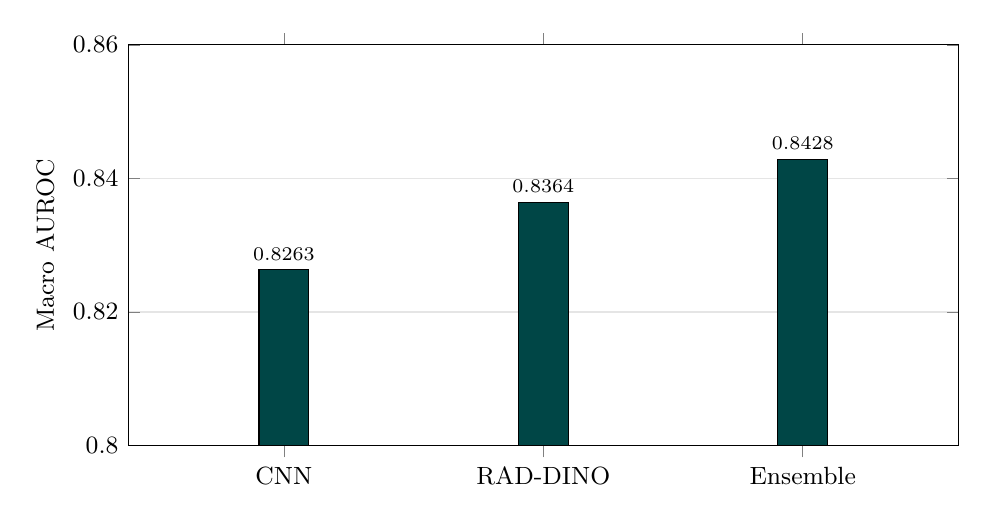
\begin{tikzpicture}
\begin{axis}[
  width=\columnwidth,
  height=0.55\columnwidth,
  ybar,
  bar width=18pt,
  ymin=0.80, ymax=0.86,
  symbolic x coords={CNN,RAD-DINO,Ensemble},
  xtick=data,
  ylabel={Macro AUROC},
  nodes near coords={\pgfmathprintnumber[precision=4,fixed]{\pgfplotspointmeta}},
  every node near coord/.append style={font=\scriptsize},
  tick label style={font=\small},
  label style={font=\small},
  ymajorgrids,
  grid style={gray!20},
  enlarge x limits=0.3,
]
\addplot[fill=teal!55!black] coordinates {(CNN,0.8263) (RAD-DINO,0.8364) (Ensemble,0.8428)};
\end{axis}
\end{tikzpicture}
\caption{Macro AUROC of the two teacher components and their calibrated average. The ensemble exceeds both single models, evidence that the CNN and RAD-DINO make partly complementary errors.}
\label{fig:teacher}
\end{figure}

\begin{table*}[t]
\centering
\caption{Paired test-set differences between the baseline systems (A $-$ B [95\% CI]). All differences are significant except those marked \ns.}
\label{tab:baseline}
\resizebox{\textwidth}{!}{%
\begin{tabular}{@{}lcccc@{}}
\toprule
Comparison & Macro AUROC & Macro AUPRC & Macro F1 & Micro F1 \\
\midrule
RAD-DINO $-$ CNN     & $+0.0101$ [$+0.0063$, $+0.0140$] & $+0.0235$ [$+0.0131$, $+0.0339$] & $+0.0249$ [$+0.0108$, $+0.0390$] & $+0.0145$ [$+0.0104$, $+0.0187$] \\
Average $-$ CNN      & $+0.0165$ [$+0.0139$, $+0.0193$] & $+0.0303$ [$+0.0229$, $+0.0379$] & $+0.0279$ [$+0.0175$, $+0.0407$] & $+0.0249$ [$+0.0217$, $+0.0283$] \\
Average $-$ RAD-DINO & $+0.0064$ [$+0.0049$, $+0.0080$] & $+0.0069$ [$+0.0028$, $+0.0113$] & $+0.0030$ [$-0.0019$, $+0.0085$]\ns & $+0.0104$ [$+0.0073$, $+0.0134$] \\
\bottomrule
\end{tabular}}
\end{table*}

The distillation criterion was also evaluated before student training. The teacher ensemble achieved a macro AUROC of 0.9165 on the training images, below the pre-specified 0.95 stop line, and distillation was therefore performed. On the training images, the teacher assigned an average probability of 0.28 to true positives and 0.03 to negatives, providing graded targets rather than reproducing the original binary labels.

\subsection{Student Performance and Statistical Comparison}

The student achieved its best validation macro AUROC at epoch 6 (0.8640, compared with 0.8598 for the CNN). After epoch 6, the student's validation loss remained nearly unchanged (0.300 to 0.301), whereas the CNN's increased from 0.305 to 0.316. The test-set improvement therefore occurred alongside an improvement on the validation split rather than appearing only on the final test set.

\Cref{tab:paired} gives the paired test-set comparisons. Relative to the CNN, the student significantly improved macro AUROC by 0.0076, macro AUPRC by 0.0158, macro F1 by 0.0163, macro recall by 0.0318, and macro precision by 0.0137. The micro-F1 difference was not significant (+0.0020, 95\% CI $[-0.0012,+0.0052]$). Importantly, these improvements were obtained at identical measured inference cost.

Relative to RAD-DINO, the student's macro AUROC was 0.0025 lower (0.8339 vs.\ 0.8364), with a 95\% CI for the paired difference of $[-0.0056,+0.0004]$ and Holm-adjusted $p=0.078$. The corresponding differences in macro AUPRC, macro F1, macro recall, and macro precision were also not significant. Micro F1 was the exception: RAD-DINO exceeded the student by 0.0126, with a 95\% CI for the student-minus-RAD-DINO difference of $[-0.0169,-0.0082]$.

The pre-specified practical-similarity margin for the primary metric was narrowly not met: the lower confidence bound of the student-minus-RAD-DINO macro-AUROC difference was $-0.0056$, compared with the margin of $-0.005$. Thus, the results support improvement over the CNN and a small, statistically non-significant macro-AUROC difference from RAD-DINO, but do not establish formal equivalence to RAD-DINO.

\begin{table*}[t]
\centering
\caption{Paired test-set differences, distilled student minus each reference (A $-$ B [95\% CI]). All differences are significant except those marked \ns.}
\label{tab:paired}
\resizebox{\textwidth}{!}{%
\begin{tabular}{@{}lccc@{}}
\toprule
Metric & Student $-$ CNN (same cost) & Student $-$ RAD-DINO (5.7$\times$ costlier) & Student $-$ Average (6.7$\times$ costlier) \\
\midrule
Macro AUROC     & $+0.0076$ [$+0.0058$, $+0.0096$] & $-0.0025$ [$-0.0056$, $+0.0004$]\ns & $-0.0089$ [$-0.0112$, $-0.0071$] \\
Macro AUPRC     & $+0.0158$ [$+0.0109$, $+0.0212$] & $-0.0077$ [$-0.0180$, $+0.0017$]\ns & $-0.0146$ [$-0.0223$, $-0.0078$] \\
Macro F1        & $+0.0163$ [$+0.0103$, $+0.0230$] & $-0.0086$ [$-0.0204$, $+0.0036$]\ns & $-0.0116$ [$-0.0218$, $-0.0026$] \\
Micro F1        & $+0.0020$ [$-0.0012$, $+0.0052$]\ns & $-0.0126$ [$-0.0169$, $-0.0082$] & $-0.0230$ [$-0.0261$, $-0.0195$] \\
Macro recall    & $+0.0318$ [$+0.0247$, $+0.0389$] & $+0.0006$ [$-0.0138$, $+0.0165$]\ns & $+0.0061$ [$-0.0060$, $+0.0175$]\ns \\
Macro precision & $+0.0137$ [$+0.0050$, $+0.0278$] & $-0.0036$ [$-0.0189$, $+0.0096$]\ns & $-0.0086$ [$-0.0202$, $+0.0002$]\ns \\
\bottomrule
\end{tabular}}
\end{table*}

\subsection{Gap Recovery Across Metrics and Findings}

The magnitude of the student's improvement can also be expressed relative to the CNN-to-RAD-DINO gap. \Cref{fig:gaprecovery} summarizes this recovery across five metrics: the student recovered 75\% of the macro AUROC gap, 67\% of the macro AUPRC gap, 65\% of the macro F1 gap and 79\% of the precision gap, and it slightly exceeded the recall gap (102\%; its macro recall of 0.4622 marginally exceeded RAD-DINO's 0.4616). These figures quantify how much of the teacher-model improvement was transferred to the lower-cost student, without implying equivalence across all metrics.

\begin{figure}[t]
\centering
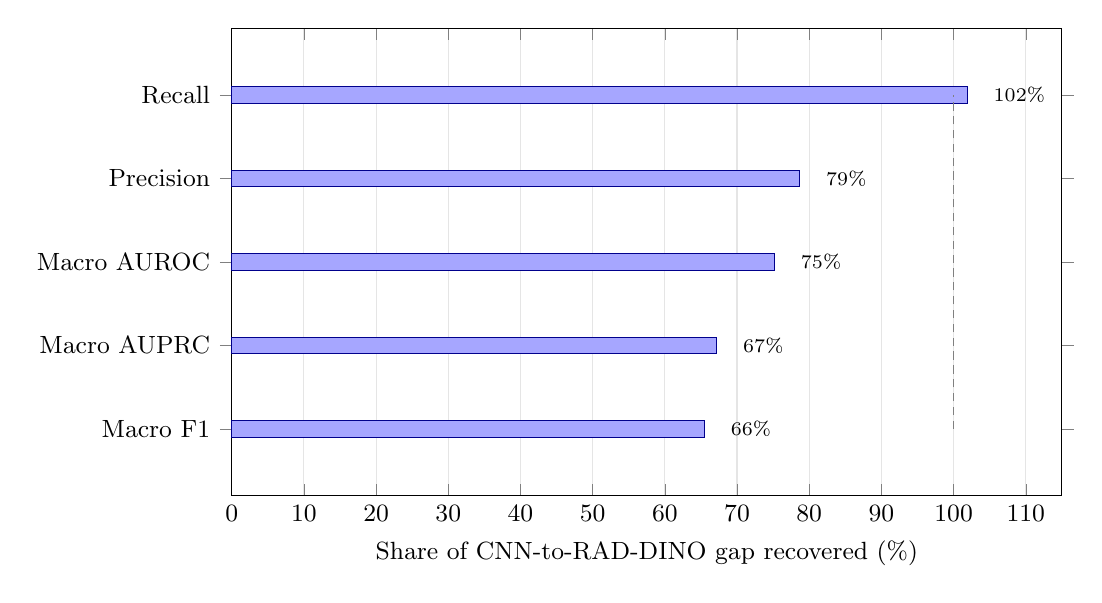
\begin{tikzpicture}
\begin{axis}[
  width=\columnwidth,
  height=0.62\columnwidth,
  xbar,
  bar width=6pt,
  xmin=0, xmax=115,
  xlabel={Share of CNN-to-RAD-DINO gap recovered (\%)},
  symbolic y coords={Macro F1,Macro AUPRC,Macro AUROC,Precision,Recall},
  ytick=data,
  nodes near coords={\pgfmathprintnumber[precision=0]{\pgfplotspointmeta}\%},
  every node near coord/.append style={font=\scriptsize, xshift=6pt},
  tick label style={font=\small},
  label style={font=\small},
  enlarge y limits=0.2,
  xmajorgrids,
  grid style={gray!20},
  clip=false,
]
\addplot[fill=blue!35!white, draw=blue!55!black] coordinates {
  (65.5,Macro F1)
  (67.2,Macro AUPRC)
  (75.2,Macro AUROC)
  (78.7,Precision)
  (101.9,Recall)
};
\draw[densely dashed, gray] (axis cs:100,Macro F1) -- (axis cs:100,Recall);
\end{axis}
\end{tikzpicture}
\caption{Share of the CNN-to-RAD-DINO gap recovered by the distilled student, by metric. The dashed line marks full recovery (100\%); the student slightly exceeded it on recall.}
\label{fig:gaprecovery}
\end{figure}

\Cref{fig:perfinding} shows the test AUROC gain of the student over the CNN for all 14 findings, with 95\% confidence intervals from 1,000 patient-level bootstrap resamples (seed 20260922, the same procedure used for \cref{tab:paired}). Ordering is from smallest (bottom) to largest (top) point estimate. Among the eight findings where RAD-DINO led the CNN by at least 0.005, the student recovered most of the gap for Mass (94\%), Hernia (87\%, only 86 positive test images), Atelectasis (80\%) and Cardiomegaly (70\%); recovery was smaller for Fibrosis (68\%), Pleural thickening (37\%), Pneumothorax (31\%) and Emphysema (19\%). On the remaining six findings RAD-DINO's lead over the CNN was under 0.005, so gap recovery is not a meaningful ratio there; even so, the student improved over the CNN on all six, from +0.0013 AUROC on Effusion to +0.0076 on Pneumonia, and on four of them (Infiltration, Consolidation, Edema, Pneumonia) it exceeded both single models in point estimate. The 95\% CI excludes zero for 13 of the 14 findings; the exception is Effusion (+0.0013, 95\% CI $[-0.0002,+0.0027]$). These per-finding intervals are exploratory and not corrected for multiplicity.

\begin{figure}[t]
\centering
\begin{tikzpicture}
\begin{axis}[
  width=\columnwidth,
  height=1.3\columnwidth,
  xbar,
  bar width=4pt,
  xmin=-0.006, xmax=0.062,
  xlabel={Student $-$ CNN AUROC (95\% CI)},
  symbolic y coords={Effusion,Infiltration,Emphysema,Nodule,Mass,Atelectasis,Edema,Pneumothorax,Consolidation,Cardiomegaly,Pleural thickening,Pneumonia,Fibrosis,Hernia$^\dagger$},
  ytick=data,
  yticklabel style={font=\scriptsize},
  tick label style={font=\scriptsize},
  label style={font=\small},
  nodes near coords={+\pgfmathprintnumber[precision=4,fixed]{\pgfplotspointmeta}},
  every node near coord/.append style={font=\tiny, xshift=16pt},
  enlarge y limits={abs=3pt},
  xmajorgrids,
  grid style={gray!20},
  clip=false,
  error bars/x dir=both,
  error bars/x explicit,
  legend style={at={(0.98,0.03)}, anchor=south east, font=\scriptsize, draw=none, fill=none},
  legend cell align=left,
]
\addplot[fill=blue!55!black, error bar style={black, thin}]
  table[x=delta,y=finding,x error minus=minus,x error plus=plus] {
finding delta minus plus
Emphysema 0.0024 0.0020 0.0023
Mass 0.0052 0.0038 0.0041
Atelectasis 0.0060 0.0020 0.0022
Pneumothorax 0.0067 0.0031 0.0040
Cardiomegaly 0.0073 0.0031 0.0033
{Pleural thickening} 0.0075 0.0038 0.0040
Fibrosis 0.0132 0.0076 0.0081
{Hernia$^\dagger$} 0.0295 0.0208 0.0228
};
\addplot[fill=orange!70!black, error bar style={black, thin}]
  table[x=delta,y=finding,x error minus=minus,x error plus=plus] {
finding delta minus plus
Effusion 0.0013 0.0014 0.0014
Infiltration 0.0018 0.0018 0.0017
Nodule 0.0045 0.0034 0.0035
Edema 0.0060 0.0030 0.0030
Consolidation 0.0067 0.0035 0.0035
Pneumonia 0.0076 0.0061 0.0058
};
\legend{RAD-DINO led CNN by $\geq$0.005, RAD-DINO led CNN by $<$0.005}
\end{axis}
\end{tikzpicture}
\caption{Test-set AUROC gain of the distilled student over the CNN, for all 14 ChestX-ray14 findings, with 95\% patient-bootstrap confidence intervals. $^\dagger$Hernia has only 86 positive test images; its estimate is uncertain. The interval excludes zero for every finding except Effusion; these per-finding results are exploratory and not corrected for multiplicity.}
\label{fig:perfinding}
\end{figure}

\subsection{Prediction-Level Analysis}

The student also partially reproduced predictions that were positive under RAD-DINO but negative under the CNN. \Cref{fig:overlap} illustrates this: among 2,831 test instances in this category, the student predicted 936 (33\%) as positive. Across the test set, the student produced 582 more true positives than the CNN. At the F1-optimal thresholds, this increase in recall was accompanied by 1,857 additional false positives, with macro specificity decreasing from 0.9040 to 0.8993.

\begin{figure}[t]
\centering
\resizebox{\columnwidth}{!}{%
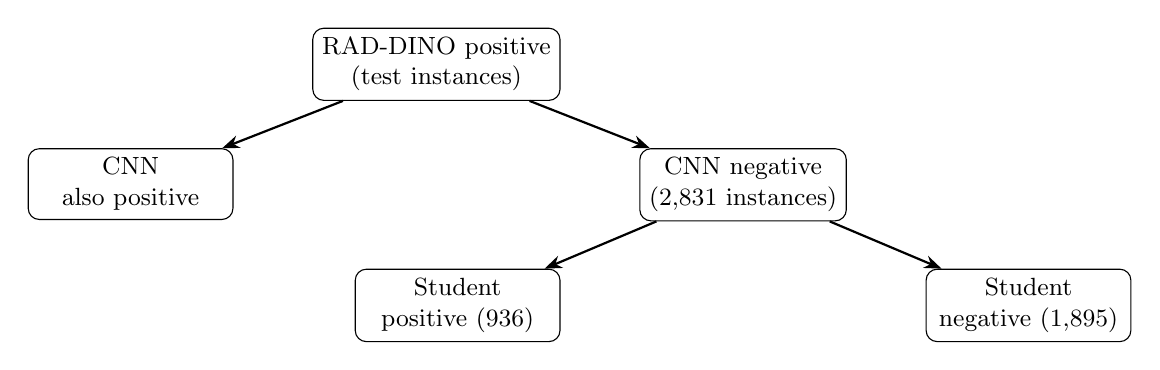
\begin{tikzpicture}[
  node distance=6mm and 10mm,
  box/.style={draw, rounded corners, align=center, minimum height=8mm, minimum width=26mm, font=\small},
  arr/.style={-{Stealth[length=2.2mm]}, thick}
]
\node[box] (rd) {RAD-DINO positive\\(test instances)};
\node[box, below left=of rd] (cp) {CNN\\also positive};
\node[box, below right=of rd] (cn) {CNN negative\\(2{,}831 instances)};
\node[box, below left=of cn] (sp) {Student\\positive (936)};
\node[box, below right=of cn] (sn) {Student\\negative (1{,}895)};
\draw[arr] (rd) -- (cp);
\draw[arr] (rd) -- (cn);
\draw[arr] (cn) -- (sp);
\draw[arr] (cn) -- (sn);
\end{tikzpicture}}
\caption{Test instances where RAD-DINO predicted a finding positive and the CNN did not (2,831 instances). The distilled student recovers 936 of these (33\%) as positive, partially reproducing the foundation model's extra detections.}
\label{fig:overlap}
\end{figure}

The output correlations further characterize the relationship between the three single-network systems. Student outputs correlated 0.97 with the CNN and 0.84 with RAD-DINO, compared with 0.81 between the CNN and RAD-DINO. Thus, the student remained much closer to the CNN in its overall output structure while shifting toward the prediction pattern of RAD-DINO. These prediction-level results complement the aggregate metrics by showing that the student transferred part of the teacher ensemble's information without becoming identical to either teacher component.

% =====================================================================
\section{Discussion}
\label{sec:discussion}

\textbf{Why distillation works here.} The teacher combines two models that make partly different errors, so its soft labels carry information that neither the 0/1 labels nor either model alone provides. On training images the teacher's probabilities were graded (0.28 on average for positives, 0.03 for negatives) rather than hard. Soft targets of this kind are known to reduce overfitting to noisy labels~\cite{li2017noisy}, which is relevant for text-mined ChestX-ray14 labels~\cite{oakdenrayner2020exploring}. Two observations fit this view. The student's validation loss stayed flat where the CNN's rose, and the student gained even on noisy, look-alike findings such as Infiltration, Consolidation and Pneumonia.

\textbf{Where it helps most.} The student closed most of the gap on findings such as Mass, Atelectasis and Cardiomegaly. It closed less on Emphysema, Pneumothorax and Pleural thickening. These findings depend on fine detail or texture, which RAD-DINO sees at 518\,px while the student sees 384\,px. This is consistent with the capacity-gap literature~\cite{cho2019efficacy,mirzadeh2020teacher}, and it points to a clear next step: a higher-resolution student.

\textbf{Practical value.} The student needs one network, one input resolution and the compute of a small CNN. It is significantly more accurate than the original CNN at the same cost, and its macro AUROC is within 0.0025 of RAD-DINO at 5.7$\times$ lower batch cost. Under a limited compute budget, it is the best of the systems we tested. When compute is not a constraint, RAD-DINO or the teacher ensemble remain the most accurate choices.

\textbf{Comparison with earlier work.} Earlier CXR distillation studies also reported gains for compact students~\cite{ho2020utilizing,termritthikun2024explainable,kishore2025enhancing}. Our results extend this to a teacher built on a CXR foundation model. We do not compare absolute AUROC values with those studies, because results on different splits of ChestX-ray14 are not comparable, and the official test split used here is harder than the development data (\cref{tab:data}).

\textbf{Limitations.} Each model was trained once (seed 42), so the CIs reflect test-set sampling, not retraining variability. The teacher includes the CNN itself, and self-distillation alone can improve a network~\cite{furlanello2018born}. The student's shift toward RAD-DINO suggests that the foundation model contributes, but students trained with single-model teachers would be needed to separate the two effects. The labels are text-mined, the study uses one dataset, and the cost figures cover the forward pass only. The per-finding and error analyses were exploratory.

% =====================================================================
\section{Conclusion}
\label{sec:conclusion}

We distilled a teacher ensemble of ConvNeXt-Tiny and the chest X-ray foundation model RAD-DINO into a single ConvNeXt-Tiny. On the official NIH ChestX-ray14 test split, the distilled student improved macro AUROC from 0.8263 to 0.8339 at unchanged inference cost. It also improved AUPRC, F1, recall and precision. It came within 0.0025 macro AUROC of RAD-DINO, a difference that was not significant, while running 5.7$\times$ faster in batch inference, and it closed about three quarters of the AUROC gap between the two models. Knowledge distillation is therefore a simple and effective way to bring much of a foundation model's accuracy to a small, fast CNN. Future work should repeat the study with several seeds, compare single-model teachers, train a higher-resolution student and evaluate on an external dataset.

% =====================================================================
\bibliographystyle{IEEEtran}
\bibliography{references}

\end{document}
